\documentclass{article}
\usepackage{graphicx}
\usepackage[margin=1in]{geometry}

\begin{document}

\begin{table}
\centering
\caption{Reduced $\chi^2$: 0.7}
\begin{tabular}{| c | c |}
\hline
$P$ (days) & $71.69028^{+0.00055}_{-0.00056}$ \\
\hline
$t_{tran}$ (days) & $43072.572^{+0.075}_{-0.071}$ \\
\hline
$\sqrt{e} cos\omega$ & $-0.0002^{+0.0016}_{-0.0023}$ \\
\hline
$\sqrt{e} sin\omega$ & $0.0005^{+0.0024}_{-0.0014}$ \\
\hline
$K_1$ (km/s) & $30.090^{+0.083}_{-0.082}$ \\
\hline
$\gamma_{1} (km/s)$ & $1.86^{+0.63}_{-0.63}$ \\
\hline
$\gamma_{2} (km/s)$ & $1.78^{+0.26}_{-0.26}$ \\
\hline
$\gamma_{3} (km/s)$ & $1.29^{+0.45}_{-0.44}$ \\
\hline
$\gamma_{4} (km/s)$ & $0.72^{+0.14}_{-0.14}$ \\
\hline
$\gamma_{5} (km/s)$ & $0.974^{+0.090}_{-0.090}$ \\
\hline
$\gamma_{6} (km/s)$ & $0.69^{+0.17}_{-0.17}$ \\
\hline
$\gamma_{7} (km/s)$ & $0.40^{+0.14}_{-0.14}$ \\
\hline
$\sigma^2_{j,1} (km/s)^2$ & $0.40^{+0.38}_{-0.29}$ \\
\hline
$\sigma^2_{j,2} (km/s)^2$ & $0.28^{+0.35}_{-0.20}$ \\
\hline
$\sigma^2_{j,3} (km/s)^2$ & $0.43^{+0.36}_{-0.30}$ \\
\hline
$\sigma^2_{j,4} (km/s)^2$ & $0.123^{+0.152}_{-0.086}$ \\
\hline
$\sigma^2_{j,5} (km/s)^2$ & $0.029^{+0.047}_{-0.022}$ \\
\hline
$\sigma^2_{j,6} (km/s)^2$ & $0.074^{+0.141}_{-0.056}$ \\
\hline
$\sigma^2_{j,7} (km/s)^2$ & $0.096^{+0.138}_{-0.066}$ \\
\hline
$e$ & $0.0022^{+0.0024}_{-0.0015}$ \\
\hline
$\omega$ (deg) & $55^{+85}_{-171}$ \\
\hline
\end{tabular}
\end{table}

\begin{figure}[!htb]
\centering
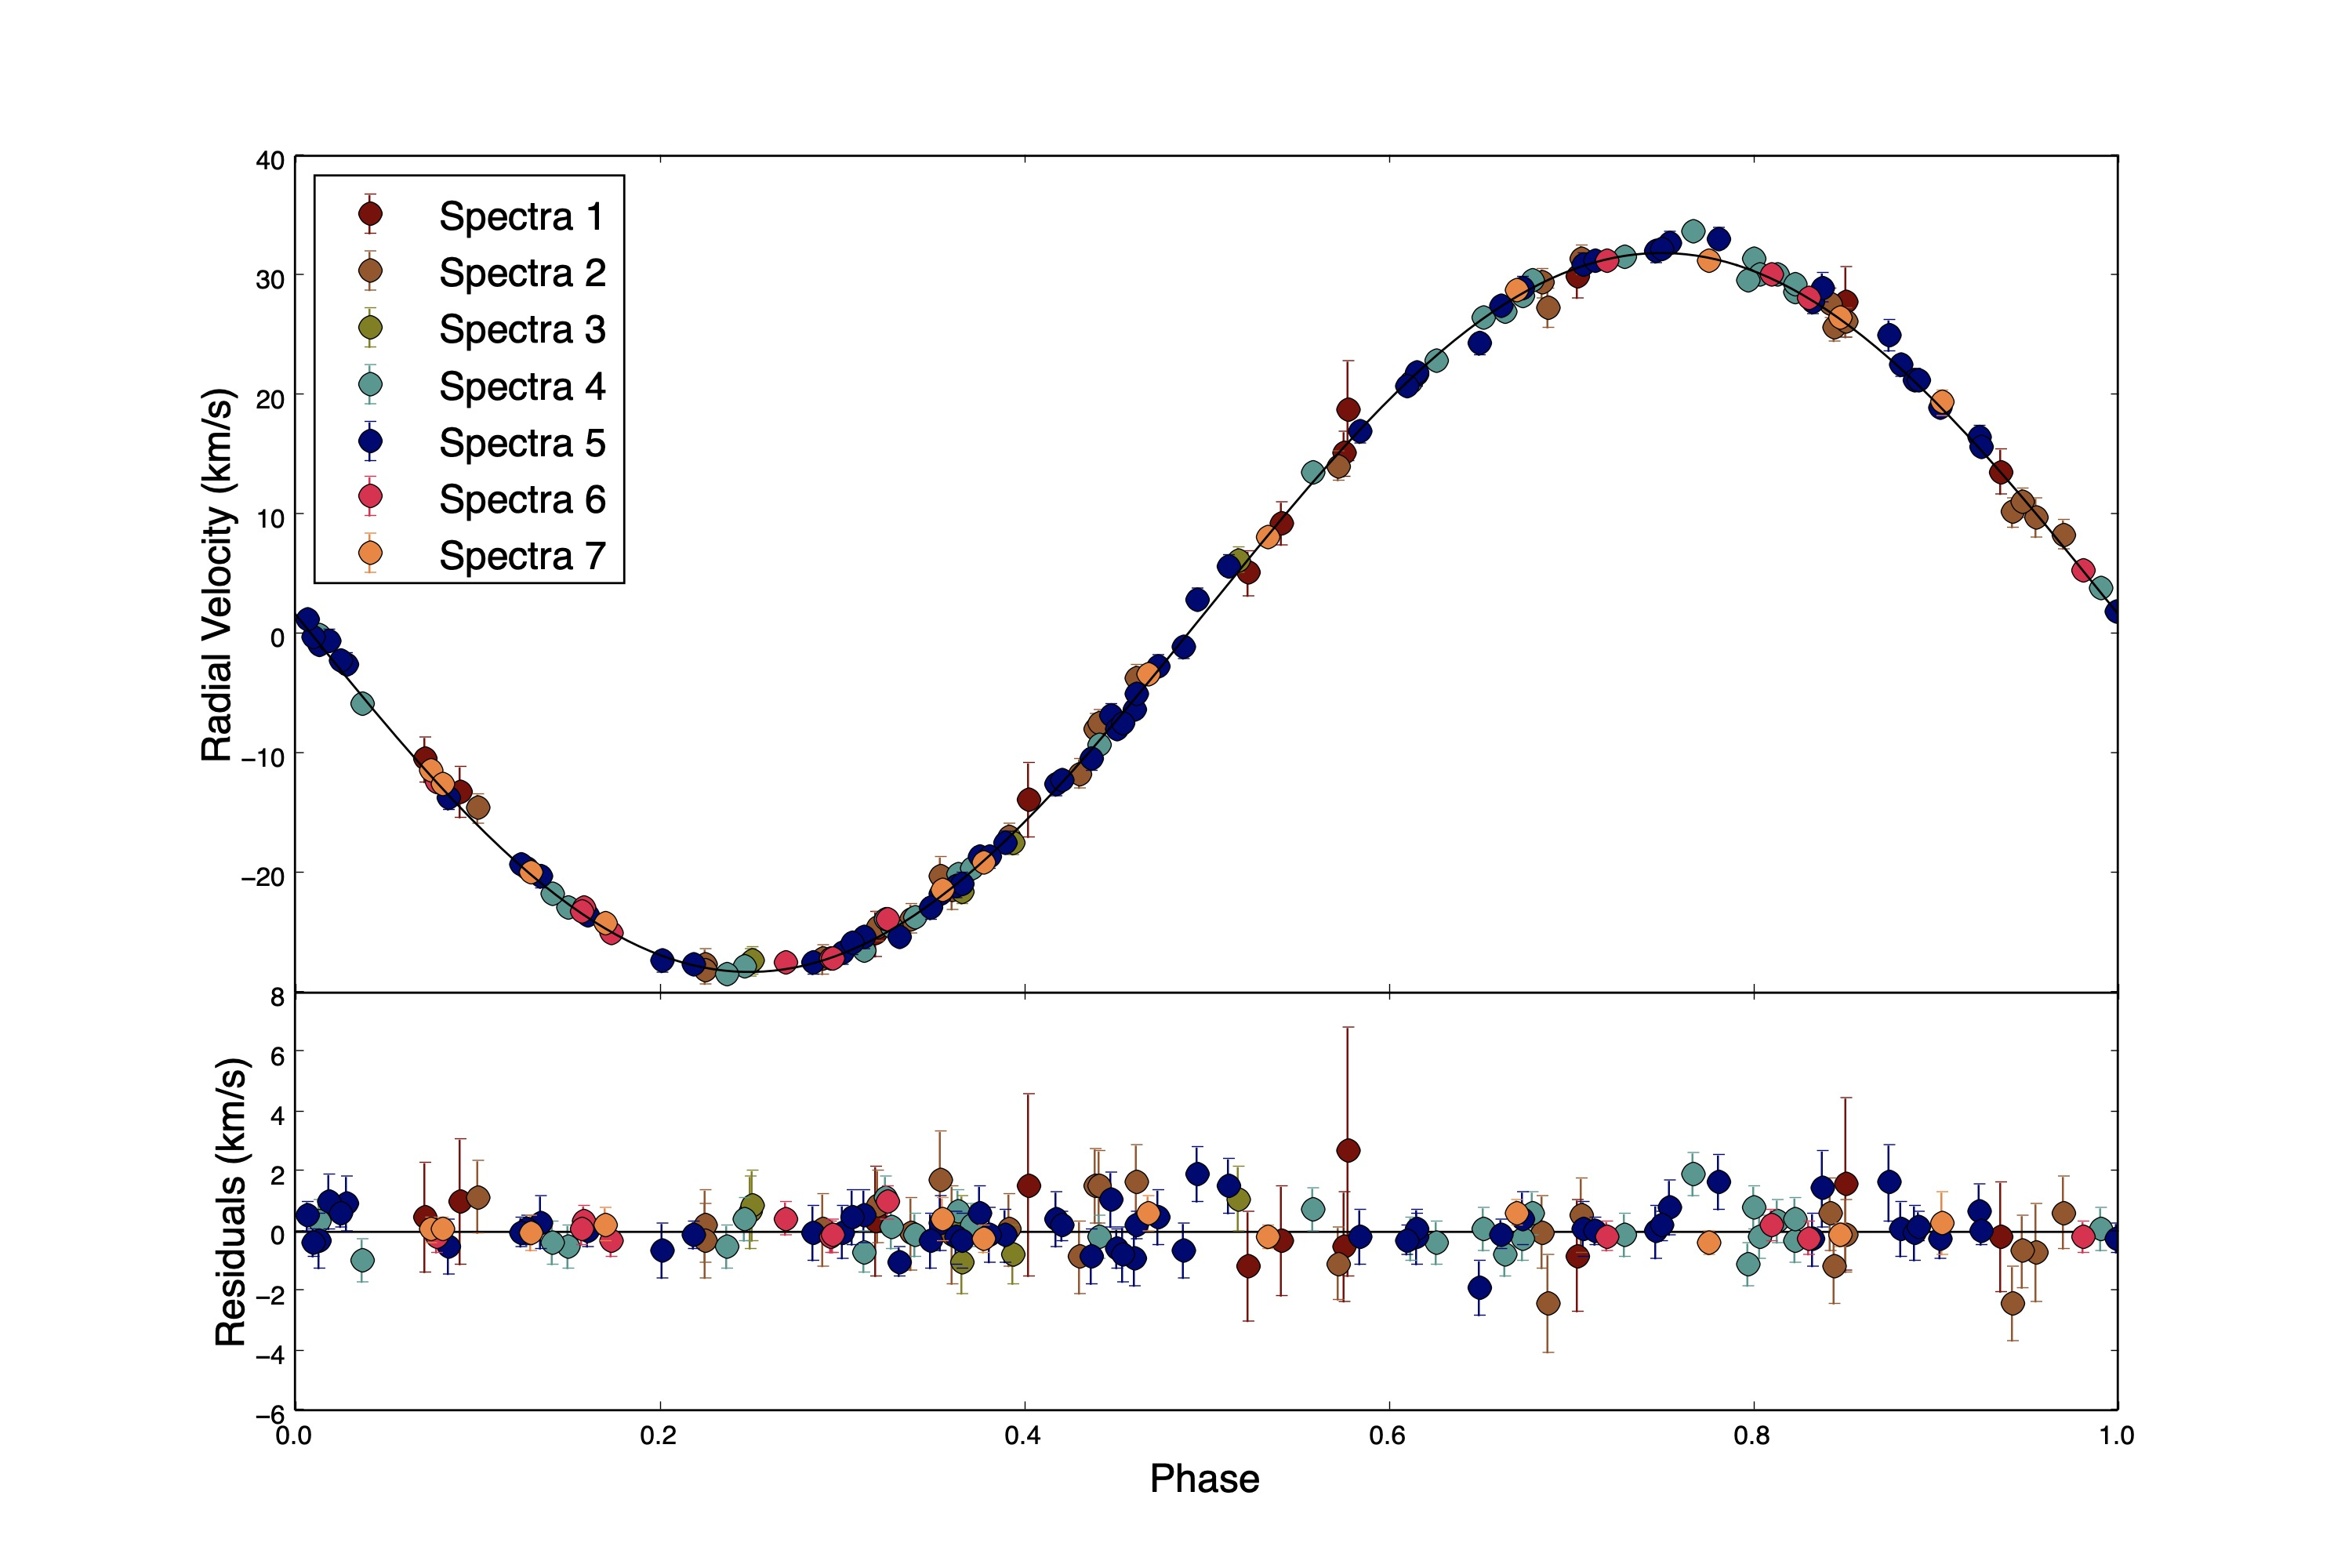
\includegraphics[width=\textwidth]{RVfit_100000_gammas.jpg}
\caption{RV fit to median MCMC parameters. RMS residual velocity of 0.77$\rm{km \: s^{-1}}$.}
\end{figure}

\begin{figure}[!htb]
\centering
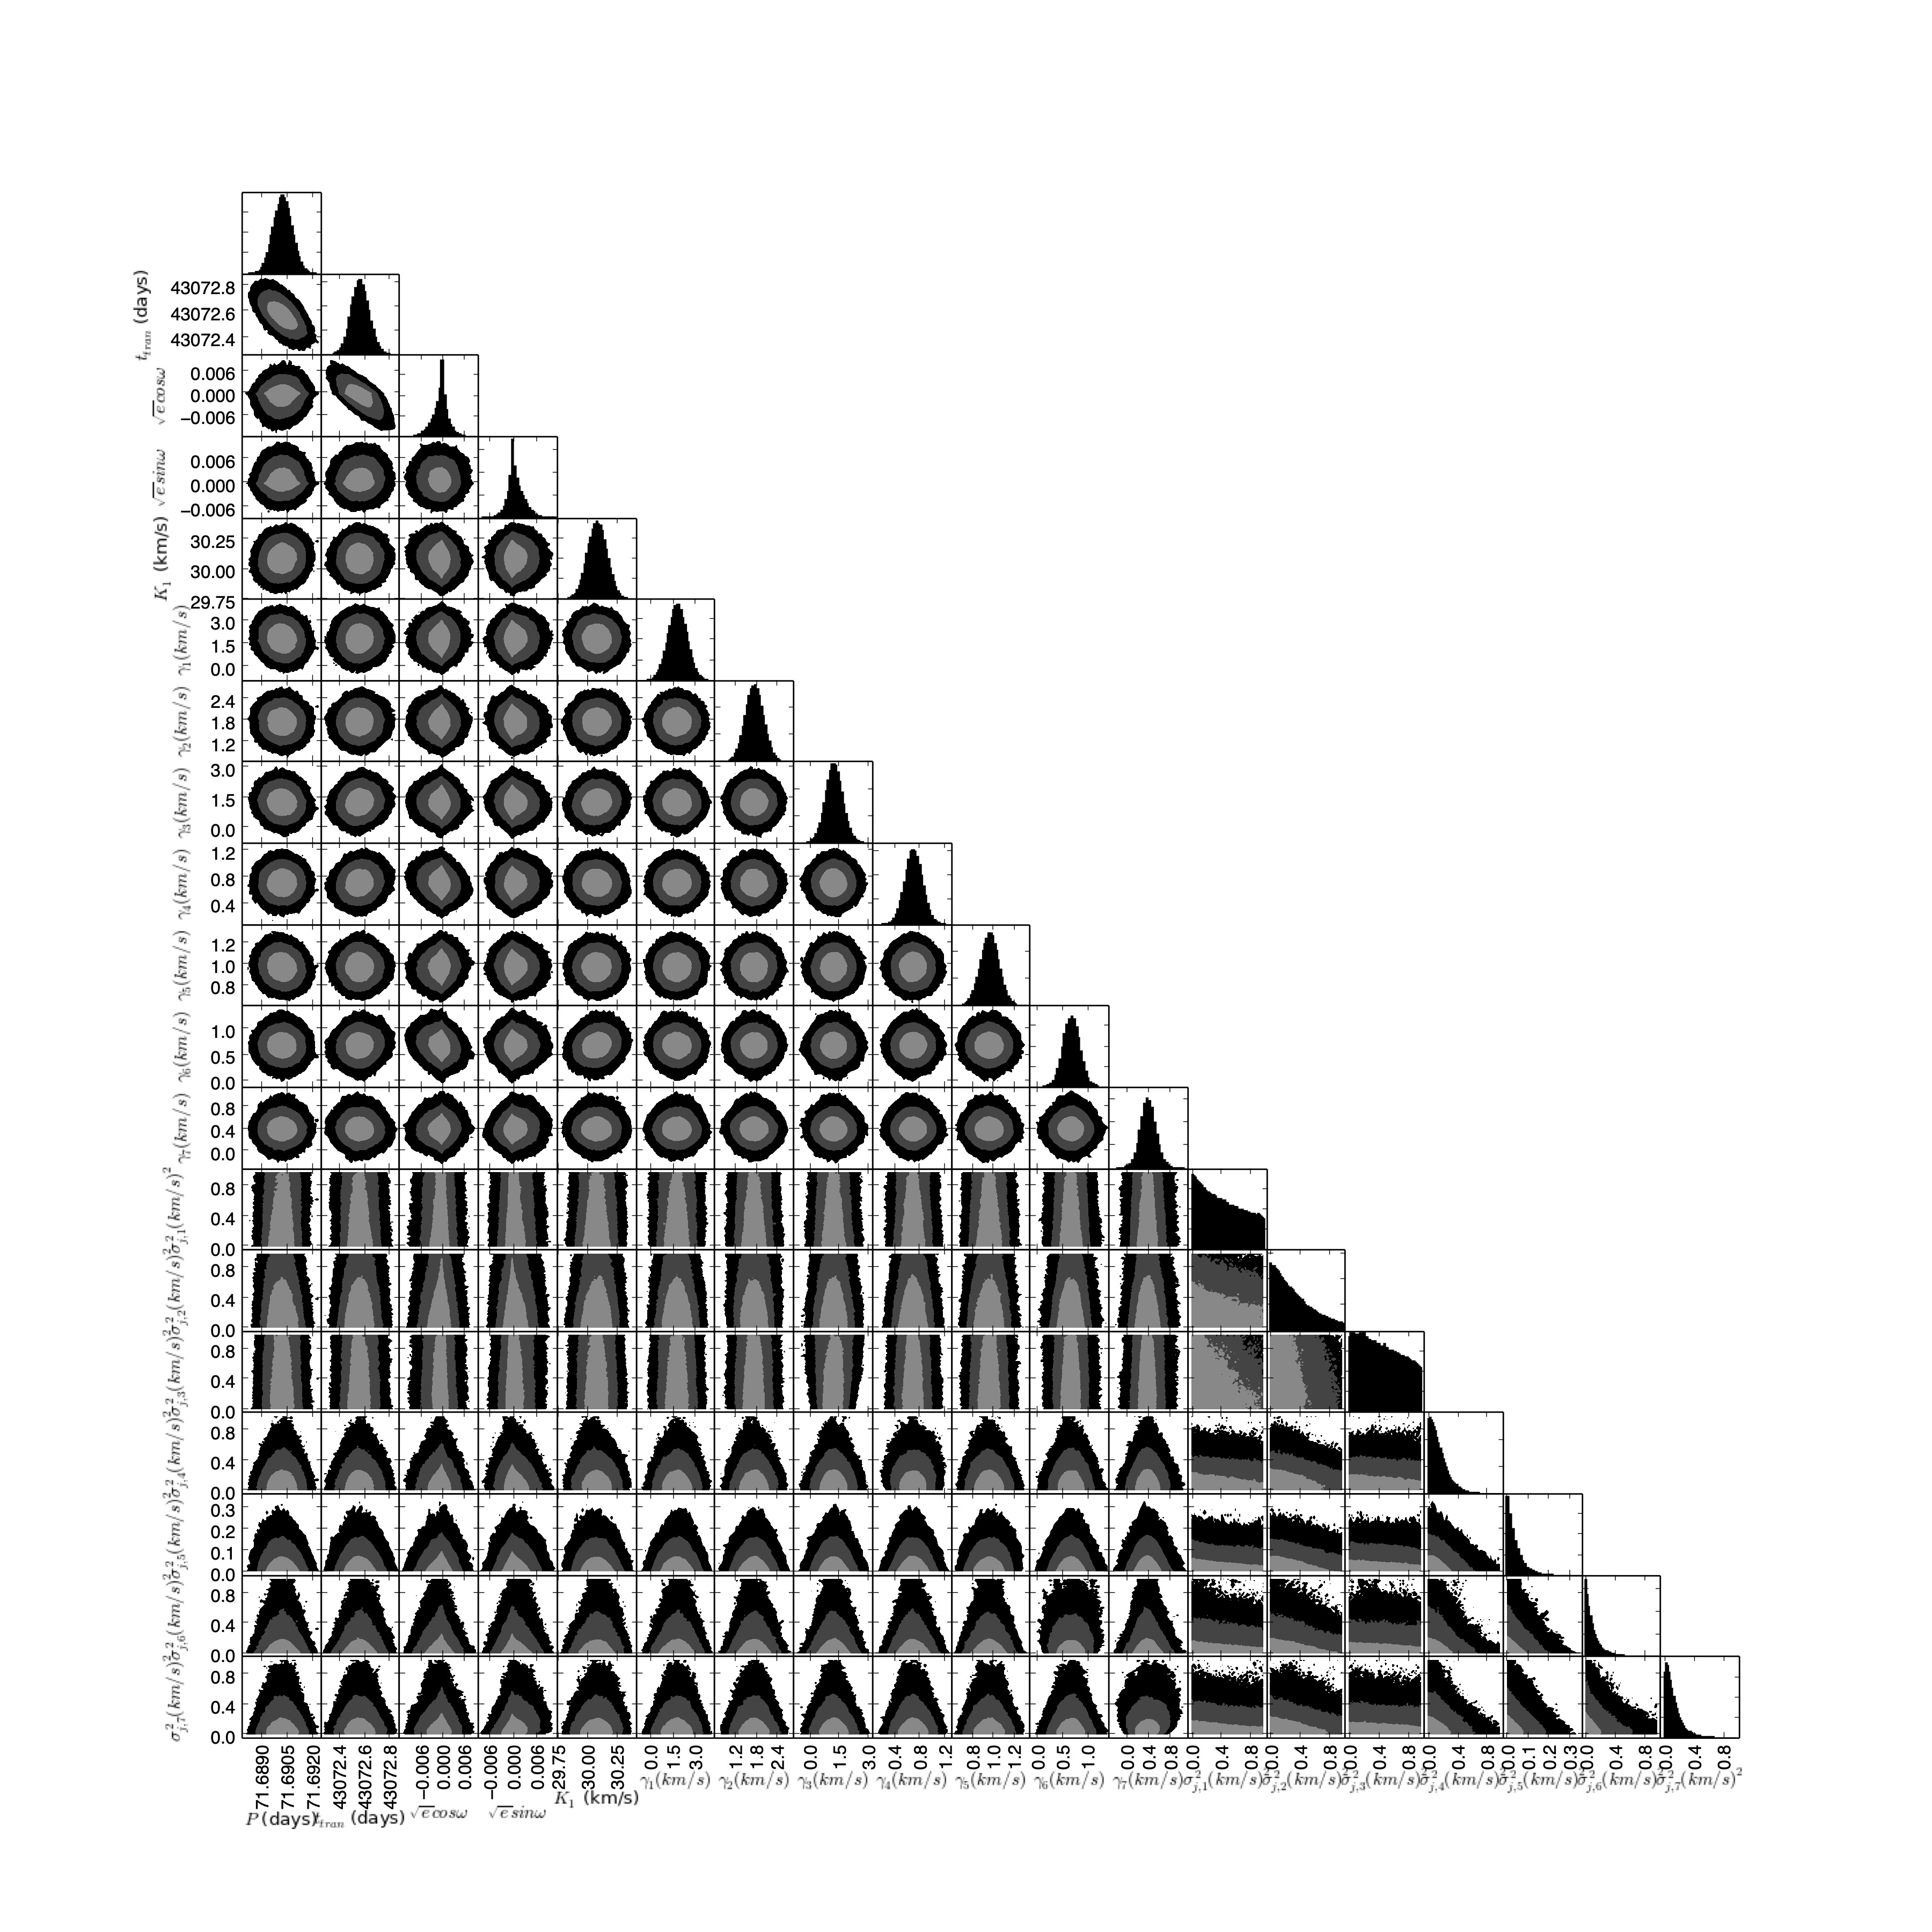
\includegraphics[width=\textwidth]{corner_100000_gammas.jpg}
\caption{Contour plots showing the $1 \sigma$, $2 \sigma$, and $3 \sigma$ constraints on pairs of parameters for the MCMC model.}
\end{figure}

\begin{figure}[!htb]
\centering
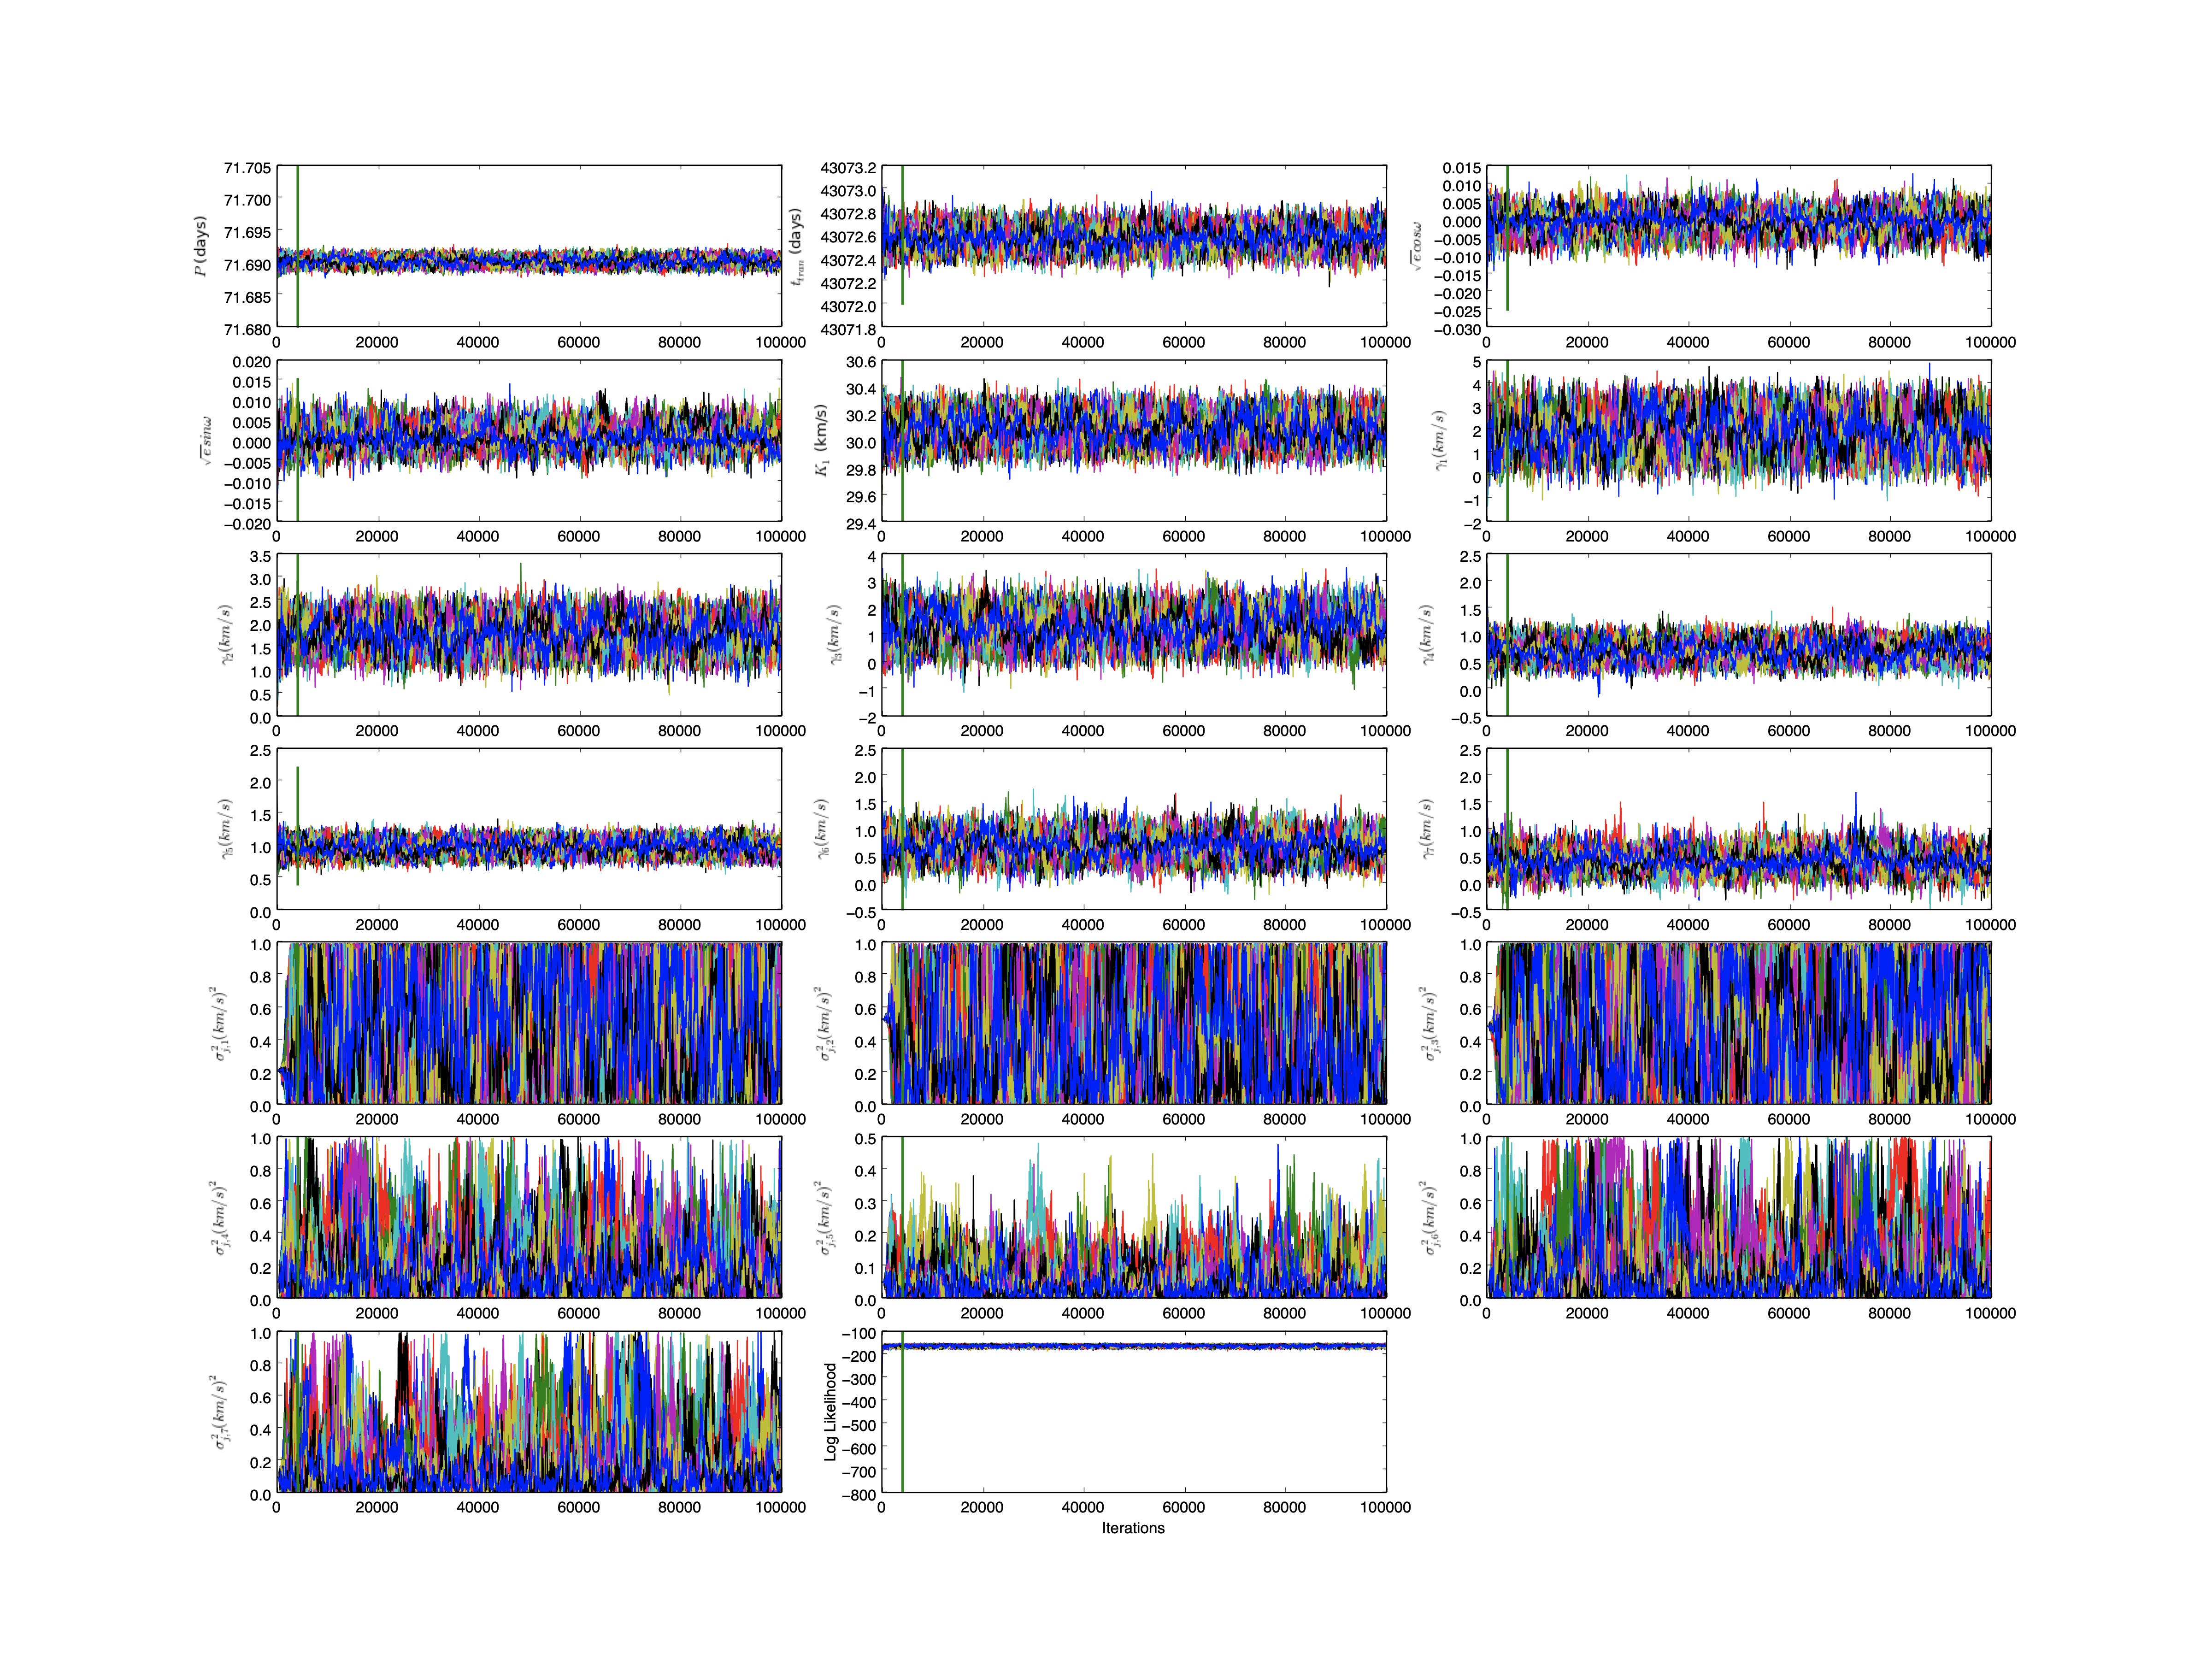
\includegraphics[width=\textwidth]{chainPlot_100000_gammas.jpg}
\caption{MCMC chains for all 50 walkers. Green line is burnout: 4000 steps.}
\end{figure}

\end{document}